% Author: Alejandro Santomé Valverde

\chapter{Fundamentals of Programmable Integrated Photonics} \label{chap:fundamentals}

\section{Fundamentals of Integrated Photonics} \label{sec:fundamentals-int_photonics}

Integrated photonics aims to generate, guide, manipulate, and detect optical signals within a 
compact and scalable platform by integrating multiple photonic components on a single substrate. 
By leveraging waveguiding structures with high refractive index contrast, photonic integrated 
circuits enable strong optical confinement and precise control of light propagation over 
centimeter-scale distances within chip-scale footprints. This approach provides a robust and 
reproducible alternative to bulk and fiber-based optical systems, while benefiting from wafer-scale 
fabrication and compatibility with semiconductor manufacturing processes 
\cite{sorefPresentFutureSilicon2006,thomsonRoadmapSiliconPhotonics2016}.

The fundamental building block of integrated photonics is the optical waveguide, which confines 
light through total internal reflection enabled by the refractive index contrast between a 
high-index core and a lower-index cladding. Depending on geometry and wavelength, waveguides may 
support single-mode or multi-mode propagation. The propagation of light along a guided mode is 
described by its propagation constant $\beta$, related to the effective refractive index 
$n_{\mathrm{eff}}$ as:

\begin{equation}
\beta = k_0 n_{\mathrm{eff}},
\end{equation}

where $k_0 = 2\pi / \lambda$ is the free-space wavenumber and $\lambda$ is the optical wavelength. 
The accumulated optical phase over a waveguide section of length $L$ is therefore given by:

\begin{equation}
\phi = \beta L = \frac{2\pi}{\lambda} n_{\mathrm{eff}} L.
\end{equation}

Controlled phase accumulation constitutes the physical basis of interferometric and resonant 
devices, which are widely used in integrated photonic circuits.

The main physical building blocks encountered in integrated photonics are summarized in 
Fig.~\ref{fig:ch2-photonics_summary}. These include waveguide confinement and guided modes, 
representative passive components for power distribution and routing, and interferometric or 
resonant structures enabling phase-sensitive functionality.

\begin{figure}[t]
    \centering
    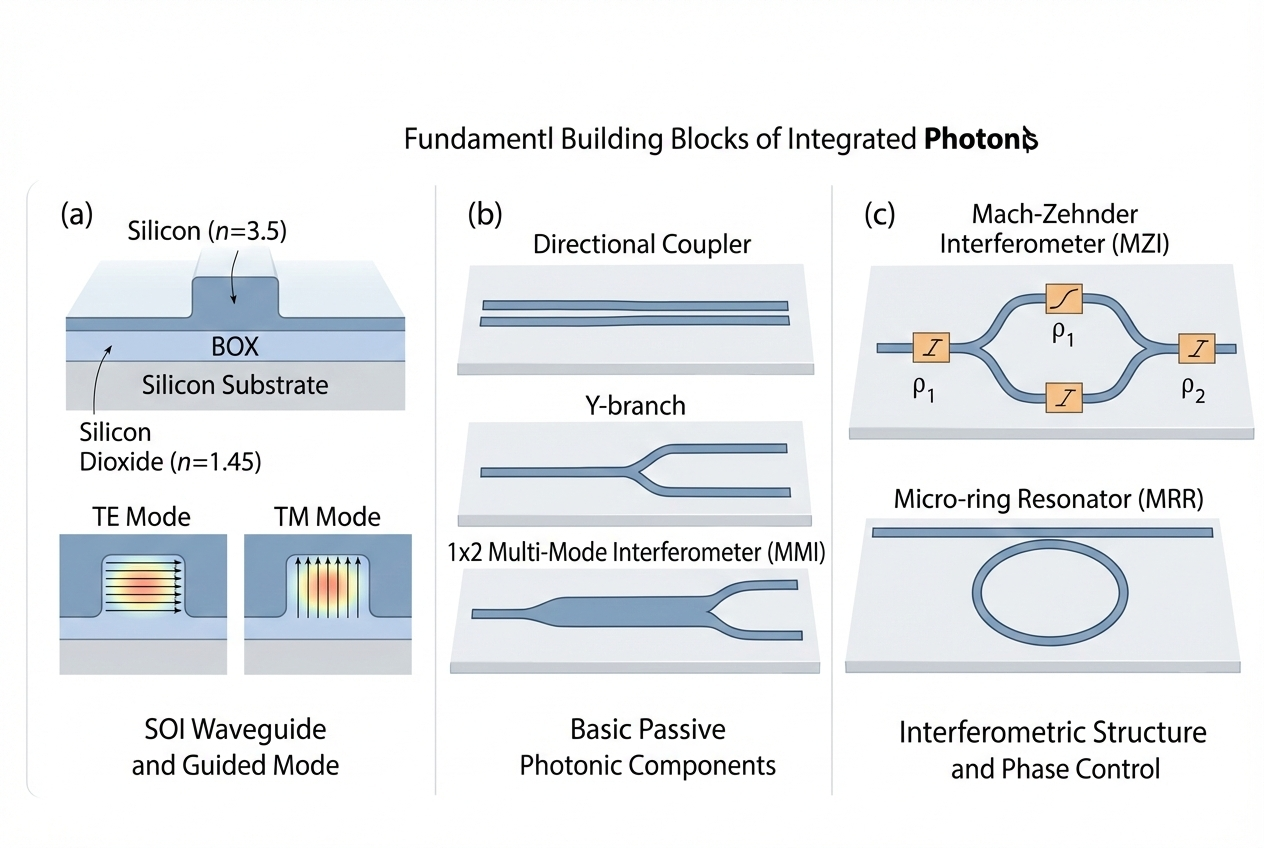
\includegraphics[width=\linewidth]{figures/ch2-photonics_summary.png}
    \caption{Fundamental building blocks of integrated photonics. 
    (a) Cross-section of a generic silicon-on-insulator (SOI) waveguide and representation of the 
    fundamental TE and TM guided modes. 
    (b) Examples of passive photonic components including a directional coupler, a Y-branch, and 
    a 1x2 multi-mode interferometer (MMI). 
    (c) Mach-Zehnder interferometer (MZI) and a micro-ring resonator (MRR).}
    \label{fig:ch2-photonics_summary}
\end{figure}

Different material platforms have been developed to implement integrated photonic circuits, 
including silicon, silicon nitride, and III-V semiconductor technologies. The choice of platform 
determines key parameters such as refractive index contrast, propagation loss, dispersion, thermal 
response, and compatibility with active functionalities. These technological aspects directly 
influence the achievable integration density, power consumption, and scalability of photonic 
circuits \cite{blumenthalSiliconNitrideSilicon2018,bogaertsSiliconPhotonicsCircuit2018}.

From a functional perspective, integrated photonic circuits are composed of passive elements that 
define optical paths and spectral responses, and active elements that enable dynamic control of 
optical signals. Phase shifters, modulators, and photodetectors allow external electrical signals 
to modify or monitor the optical state of the circuit. As the number of components increases, the 
interplay between optical confinement, phase control, losses, and fabrication variability becomes 
increasingly critical.

Loss mechanisms play a central role in determining the scalability of integrated photonic circuits. 
Propagation losses due to material absorption, sidewall roughness, and scattering, together with 
excess losses introduced by bends, couplers, and crossings, accumulate as circuit depth increases
\cite{suScalabilityLargeScalePhotonic2023}. In large-scale circuits, loss accumulation limits 
usable complexity and directly impacts signal-to-noise ratio and energy efficiency.

In summary, integrated photonics relies on controlled light confinement, phase manipulation, and 
low-loss propagation within planar waveguide platforms. These physical principles provide the 
foundation upon which specific technological implementations and programmable circuit architectures 
are built. The following sections introduce silicon photonics as the dominant integration platform, 
and subsequently discuss the building blocks and architectures that enable large-scale programmable 
photonic systems.




\section{Introduction to Silicon Photonics} \label{sec:silicon_photonics}

Silicon photonics has emerged over the past two decades as the leading platform for large-scale 
photonic integration. By leveraging the mature fabrication infrastructure of the microelectronics 
industry, silicon photonics enables the realization of complex photonic integrated circuits
with high reproducibility, scalability, and cost efficiency 
\cite{sorefPresentFutureSilicon2006,thomsonRoadmapSiliconPhotonics2016}.

The central motivation behind silicon photonics is the compatibility with complementary 
metal-oxide-semiconductor (CMOS) manufacturing processes. This compatibility allows photonic 
devices to be fabricated using advanced lithographic tools and wafer-scale processing techniques 
originally developed for electronic integrated circuits. As a result, silicon photonics benefits 
from high fabrication precision, tight dimensional control, and the possibility of co-integration 
with electronic control circuitry.

Beyond manufacturing advantages, silicon offers favorable optical properties in the near-infrared 
wavelength range, particularly around the telecommunication bands at 1.3~$\mu$m and 1.55~$\mu$m. 
In this spectral region, silicon exhibits low material absorption while maintaining a high 
refractive index ($n \approx 3.48$ at 1550~nm), enabling strong optical confinement when combined 
with lower-index materials such as silicon dioxide. This high index contrast supports compact 
waveguides, tight bending radii, and dense integration.

Silicon photonics has found widespread adoption in applications including optical interconnects 
for data centers, high-speed optical transceivers, microwave photonics, sensing, and emerging 
computing paradigms. The platform supports both passive and active functionalities. While silicon 
itself lacks a strong second-order electro-optic effect, efficient modulation can be achieved 
through carrier-based mechanisms such as plasma dispersion, and photodetection can be implemented 
via heterogeneous integration with germanium. Furthermore, hybrid and heterogeneous integration 
with III-V materials enables on-chip light sources, addressing silicon's indirect bandgap limitation.

Despite these advantages, silicon photonics also presents challenges. High index contrast increases 
sensitivity to fabrication variations and sidewall roughness, potentially leading to scattering 
losses and performance variability \cite{bogaertsSilicononInsulatorSpectralFilters2010}. Thermal 
sensitivity due to the relatively large thermo-optic coefficient of silicon introduces additional 
considerations for stability and power consumption in large-scale circuits. These aspects become 
particularly relevant in complex and programmable photonic systems.

Among the different technological implementations of silicon photonics, the silicon-on-insulator 
(SOI) platform has become the standard substrate configuration for high-index-contrast integrated 
photonics. The following subsection describes the SOI platform in detail, including its layer 
structure, optical confinement properties, and implications for device design.

\subsection{The Silicon-on-Insulator (SOI) Platform}
\label{sub:optical_wg}

The silicon-on-insulator (SOI) platform consists of a thin crystalline silicon device layer 
separated from a silicon substrate by a buried oxide (BOX) layer, typically made of silicon 
dioxide (SiO$_2$). The silicon device layer, with thicknesses commonly ranging from 220~nm to 
300~nm in standard photonic processes, defines the core material for optical waveguides, while 
the BOX layer provides vertical optical isolation from the substrate.

This layered structure creates a high refractive index contrast between the silicon core 
($n \approx 3.48$ at 1550~nm) and the surrounding oxide ($n \approx 1.44$), enabling strong 
vertical and lateral optical confinement. This effect is depicted in 
Fig.~\ref{fig:ch2-waveguide_modes}. The optical mode is tightly confined within the 
silicon core, as illustrated in Fig.~\ref{fig:ch2-waveguide_modes}(b) for TE mode and 
Fig.~\ref{fig:ch2-waveguide_modes}(c) for TM mode, resulting in submicron waveguide 
cross-sections and small bending radii, often on the order of a few micrometers.

\begin{figure}[h]
    \centering
    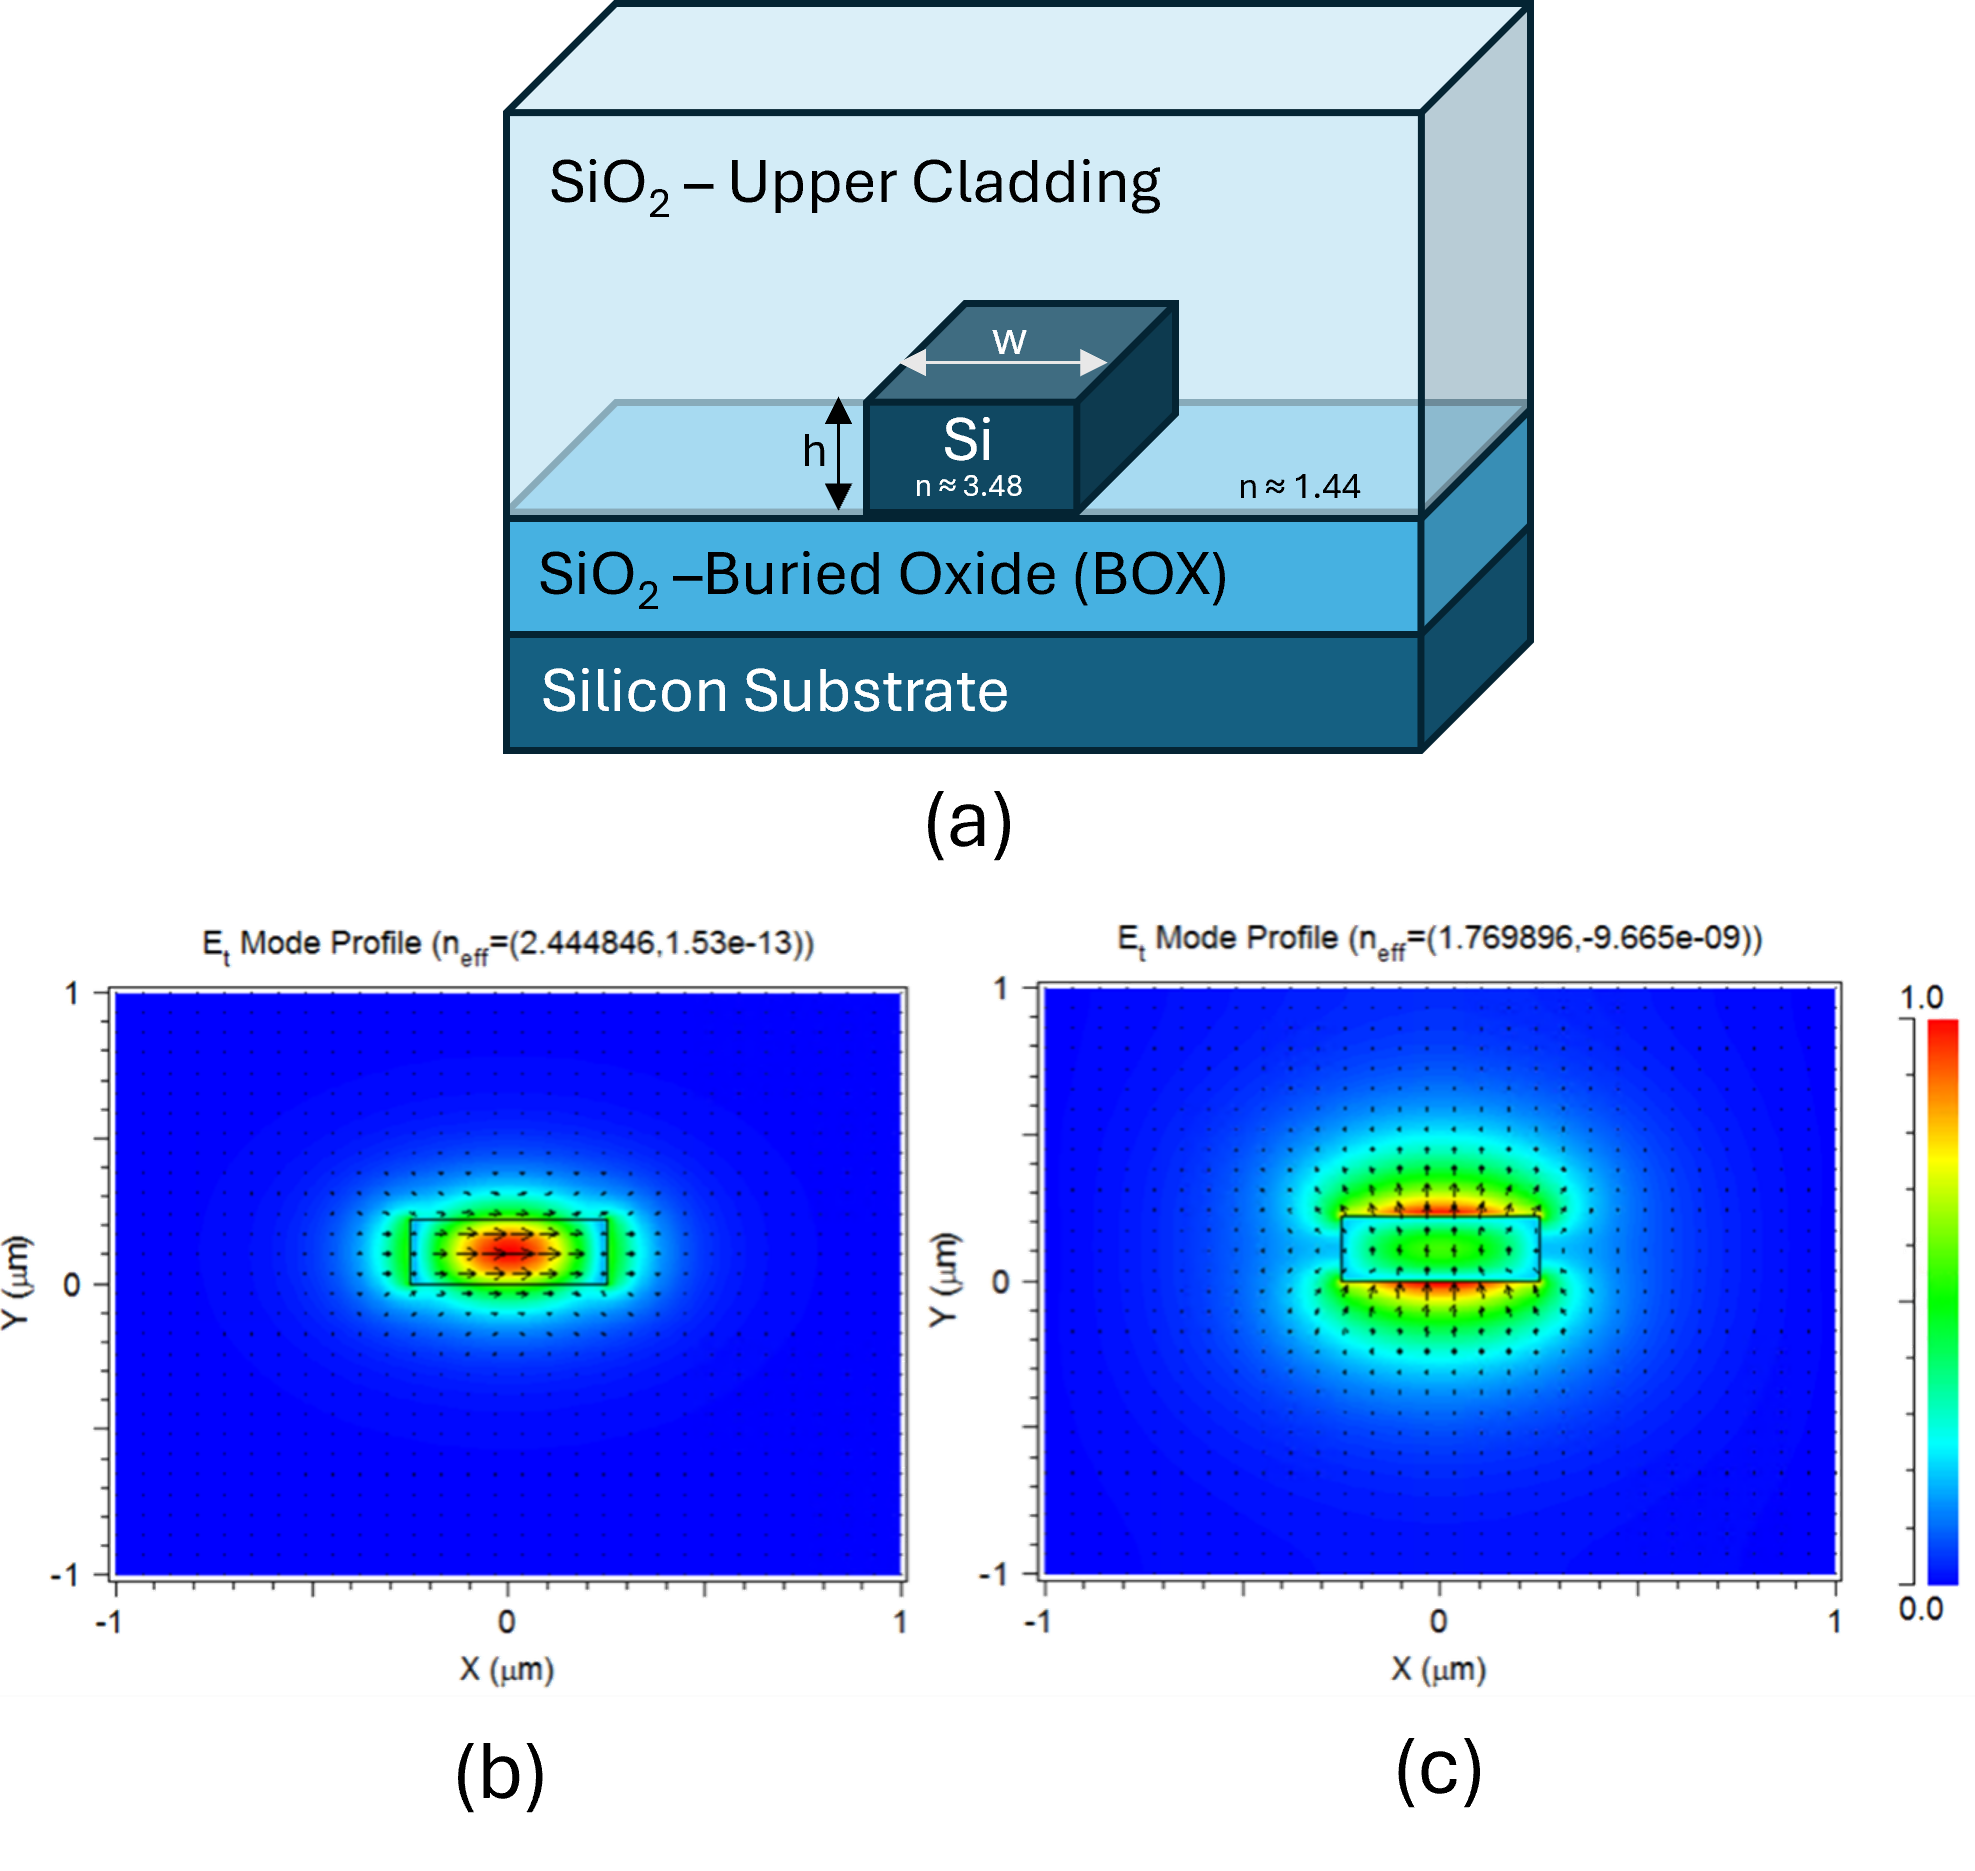
\includegraphics[width=0.7\linewidth]{figures/ch2-waveguide_modes.png}
    \caption{Standard-size silicon photonics waveguide. 
    (a) Cross-section of a generic SOI waveguide.
    (b) Simulation of fundamental TE guided mode. 
    (c) Simulation of fundamental TM guided mode.}
    \label{fig:ch2-waveguide_modes}
\end{figure}



The high confinement achievable in SOI waveguides enables compact interferometric and 
resonant devices, high integration density, and enhanced light-matter interaction. However, 
it also increases sensitivity to sidewall roughness and dimensional variations, making fabrication 
tolerances a critical design parameter. Small deviations in waveguide width or thickness can 
induce noticeable shifts in effective refractive index and device response.

Standard SOI photonic platforms are typically categorized according to device layer thickness. 
The most common configuration for telecommunications applications is the 220~nm silicon device 
layer, which supports single-mode operation for waveguide widths around 450–500~nm at 1550~nm. 
Thicker silicon layers (e.g., 300~nm or above) are also used in some processes to tailor modal 
confinement and improve performance in specific applications.

Thermal effects play a significant role in SOI-based devices due to the relatively large 
thermo-optic coefficient of silicon 
($\mathrm{d}n/\mathrm{d}T \approx 1.86 \times 10^{-4}~\mathrm{K}^{-1}$) 
\cite{cocorulloThermoopticalModulation15mm1992}. While this property enables efficient 
thermo-optic phase tuning, it also introduces thermal crosstalk and power consumption challenges 
in densely integrated circuits 
\cite{wattsAdiabaticThermoopticMach2013,coenenAnalysisThermalCrosstalk2022}.

Overall, the SOI platform provides a powerful combination of strong confinement, CMOS 
compatibility, and high integration density, which has positioned it as the dominant technology 
for large-scale silicon photonic circuits. These characteristics make SOI particularly well 
suited for the realization of complex circuits composed of multiple passive and active building 
blocks, which are discussed in the next section.



\section{Building Blocks of Programmable Circuits}

Programmable photonic circuits are constructed from a combination of passive optical structures 
and active tuning elements that, when properly interconnected, enable dynamic control over light 
propagation and interference. While passive components define the static topology of the circuit, 
active elements introduce the tunability required for reconfigurability.

The fundamental reconfigurable element in programmable photonic systems is the Programmable Unit 
Cell (PUC), which combines passive coupling structures with tunable phase shifters to implement a 
fully controllable 2x2 linear optical transformation. Before introducing the PUC in detail, it is 
necessary to review the passive and active building blocks from which it is constructed.

\subsection{Fundamental Passive Building Blocks}

Passive building blocks define the static optical backbone of programmable photonic circuits. They 
determine how light is distributed, combined, routed, and coupled within the chip. Although they 
do not provide tunability by themselves, they establish the interference pathways that, when 
combined with active phase control, enable full reconfigurability.

In silicon photonics, passive components are implemented using high-index-contrast waveguides in 
the Silicon-on-Insulator platform. The strong confinement provided by the refractive index 
contrast between silicon and silicon dioxide enables compact implementations of couplers, 
interferometers, crossings, and fiber-chip interfaces. However, this high confinement also 
increases sensitivity to fabrication variations, making precise design and modeling essential.

The most relevant passive building blocks for programmable circuits are directional couplers, 
multi-mode interferometers (MMIs), waveguide crossings, grating couplers, and edge couplers.

\subsubsection*{Directional Couplers}

Directional couplers are among the most fundamental passive elements in integrated photonics. 
They rely on evanescent coupling between two waveguides placed in close proximity over a finite 
interaction length. When the separation between the waveguides is sufficiently small, the 
evanescent tails of their guided modes overlap, enabling periodic power exchange.

The evolution of optical power along the coupling region can be described using coupled-mode 
theory. For identical waveguides, the power transferred from waveguide 1 to waveguide 2 after a 
propagation length $L$ is given by

\begin{equation}
P_2(L) = P_1(0)\sin^2(\kappa L),
\end{equation}

where $\kappa$ is the coupling coefficient, determined by the modal overlap and separation 
distance. The characteristic length required for complete power transfer, known as the coupling 
length, is

\begin{equation}
L_c = \frac{\pi}{2\kappa}.
\end{equation}

By selecting the appropriate interaction length $L$, directional couplers can implement arbitrary 
fixed splitting ratios. In programmable photonic circuits, they are typically designed as balanced 
50:50 couplers ($L = L_c$), forming the basis of interferometric structures such as Mach-Zehnder 
interferometers.

Beyond power distribution, the operation of a symmetric directional coupler is more accurately 
described by its complex-valued transfer matrix $\mathbf{M}_{\text{DC}}$. This matrix relates the 
input complex field amplitudes $(E_{in,1}, E_{in,2})$ to the output amplitudes 
$(E_{out,1}, E_{out,2})$ as:

\begin{equation}
\begin{pmatrix} E_{out,1} \\ E_{out,2} \end{pmatrix} = \mathbf{M}_{\text{DC}} \begin{pmatrix} 
    E_{in,1} \\ E_{in,2} \end{pmatrix} = \begin{pmatrix} \cos(\kappa L) & -j\sin(\kappa L) \\ 
        -j\sin(\kappa L) & \cos(\kappa L) \end{pmatrix} \begin{pmatrix} E_{in,1} \\ E_{in,2} 
        \end{pmatrix}.
\label{eq:matrix_dc}
\end{equation}


For a perfectly balanced 3-dB coupler, the coupling term $\kappa L$ equals $\pi/4$, yielding a 
$\pi/2$ phase shift between the bar and cross ports. However, the performance of these components 
is highly sensitive to wavelength fluctuations and fabrication tolerances. Small stochastic 
deviations in waveguide width or gap separation modify the effective coupling coefficient 
($\kappa \pm \Delta\kappa$), resulting in an imbalanced or non-unitary matrix. In large-scale 
programmable architectures, these systematic errors propagate through the mesh, directly 
impacting the fidelity of the synthesized optical transformations 
\cite{chrostowskiSiliconPhotonicsDesign2015}.


\begin{figure}[h!]
    \centering
    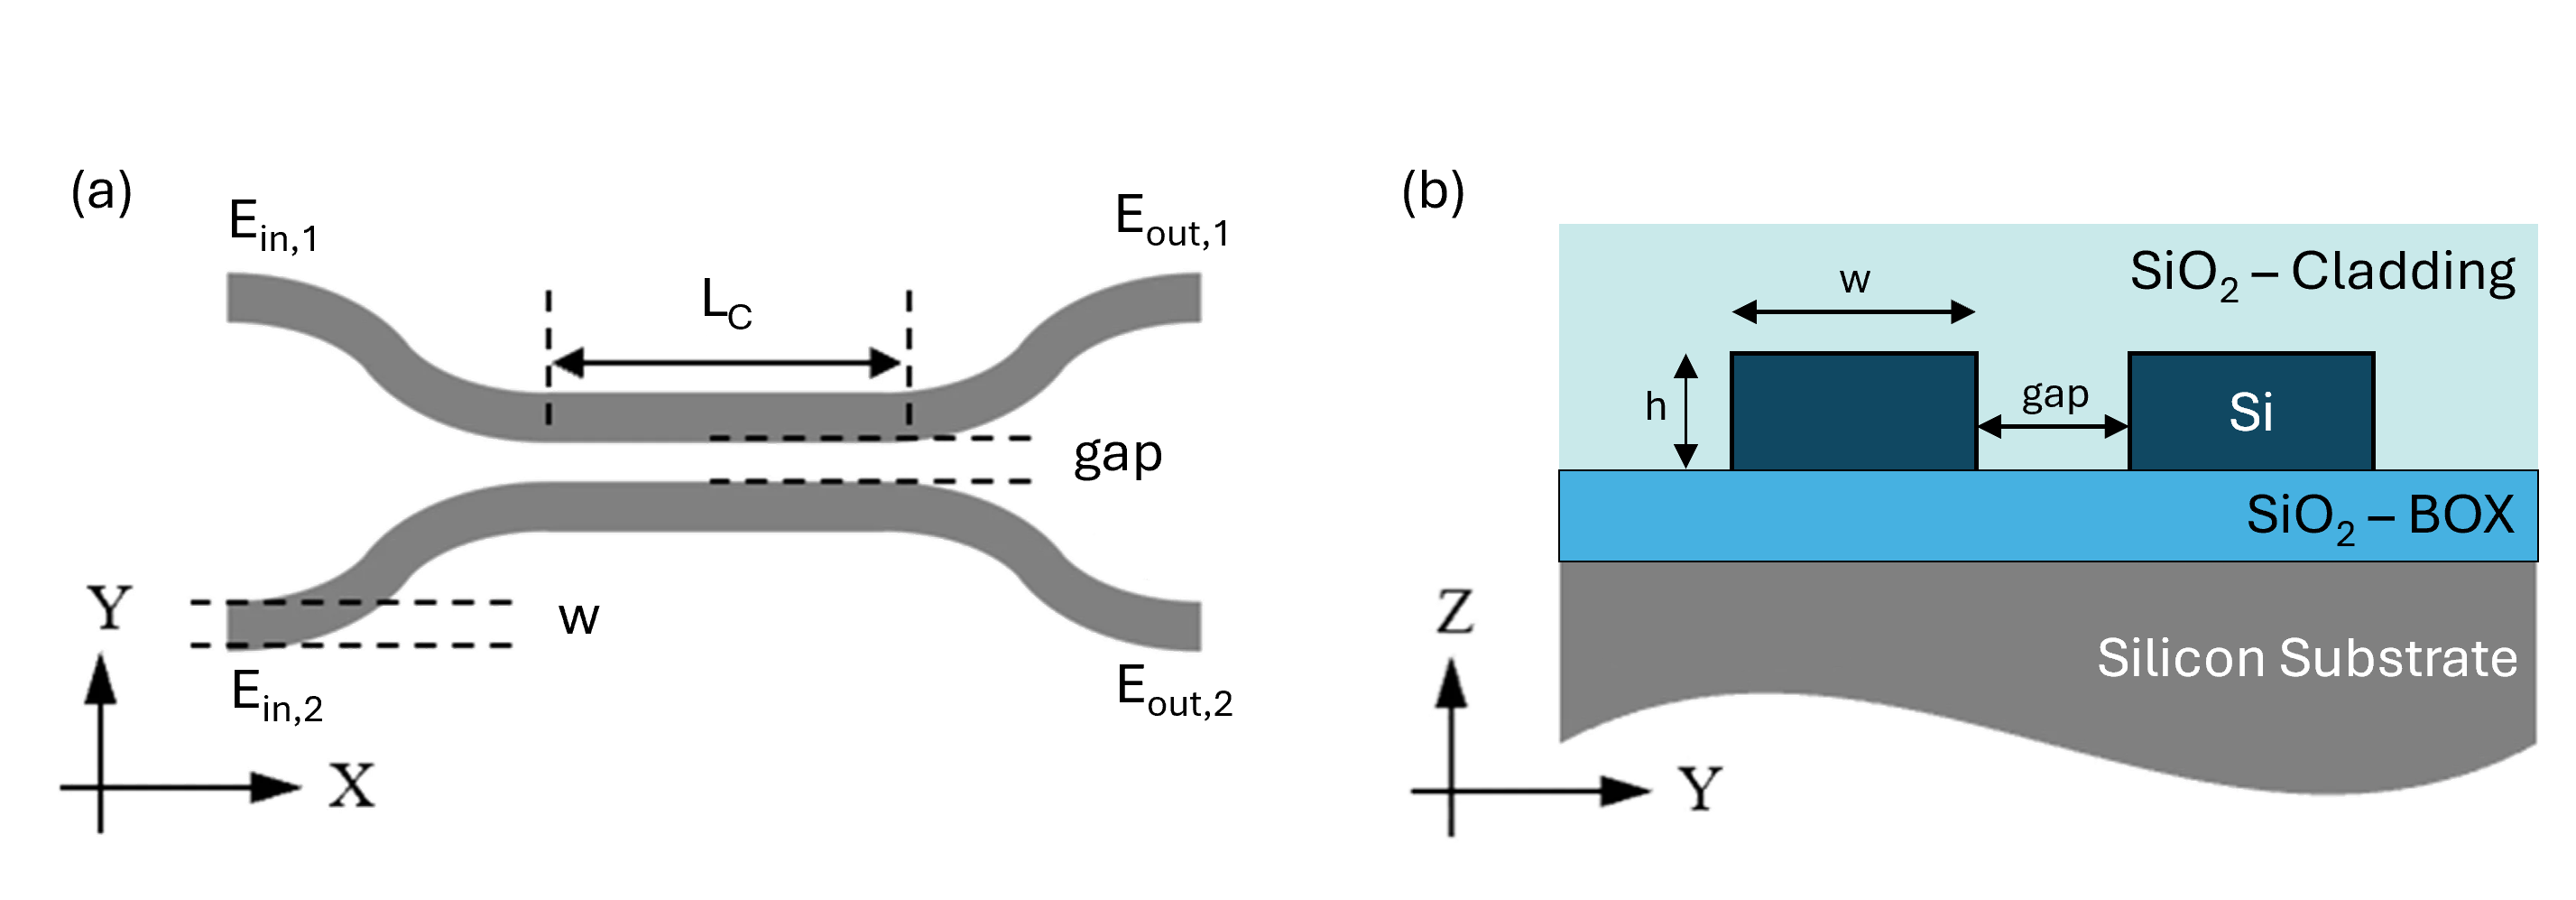
\includegraphics[width=\linewidth]{figures/ch2-directional_coupler.png}
    \caption{Schematic of a $2\times2$ symmetric directional coupler. 
    (a) Top-view illustrating the coupling length $L_c$ and the coupling gap. 
    (b) Cross-section of the coupling region in the SOI platform, where the waveguide width $w$ and 
    the gap are the critical parameters defining the coupling coefficient $\kappa$.}
\end{figure}



\subsubsection*{Multi-Mode Interferometers (MMIs)}

Multi-mode interferometers exploit the self-imaging principle in multimode waveguides. When light 
is injected into a multimode section, multiple transverse modes propagate with different 
propagation constants. The interference between these modes leads to periodic reproduction of the 
input field profile at specific distances along the propagation direction.

The characteristic beat length between the two lowest-order modes is given by

\begin{equation}
L_\pi = \frac{\pi}{\beta_0 - \beta_1},
\end{equation}

where $\beta_0$ and $\beta_1$ are the propagation constants of the fundamental and first-order 
modes, respectively. The length required to form a two-fold self-image can be approximated as

\begin{equation}
L_{\text{MMI}} \approx \frac{3L_\pi}{2}.
\end{equation}

The self-imaging mechanism in a $2\times2$ MMI results in a transfer matrix 
$\mathbf{M}_{\text{MMI}}$ that, assuming an ideal device with balanced splitting, is given by:

\begin{equation}
\mathbf{M}_{\text{MMI}} = \frac{1}{\sqrt{2}} \begin{pmatrix} 1 & e^{j\pi/2} \\ e^{j\pi/2} & 1 
\end{pmatrix} = \frac{1}{\sqrt{2}} \begin{pmatrix} 1 & j \\ j & 1 \end{pmatrix}.
\label{eq:matrix_mmi}
\end{equation}



To illustrate the self-imaging principle in a practical building block, Figure 
\ref{fig:ch2-mmi_2x2_self_imagin} shows a Beam Propagation Method (BPM) simulation of a $2\times2$ 
MMI designed for the paired interference regime. By launching the input field at a transverse 
position of $x = \pm W/6$, the device can function as either a balanced power splitter or a 
cross-coupler depending on its longitudinal dimension.

As observed in the simulation, at a distance of approximately $L_{\pi}/2$, the interference of the 
excited modes generates two symmetric images of the input field, realizing a 3-dB splitting ratio. 
Further propagation to $z \approx L_{\pi}$ results in a single reconstructed image at the opposite 
(cross) output port. It is worth noting that in high-index-contrast platforms like SOI, numerical 
calibration is essential to account for the effective width expansion due to field penetration into 
the cladding. From a fault-tolerance perspective, the stability of these imaging points against 
small lithographic deviations in $W$ is what makes the MMI a more reliable candidate than 
directional couplers for the backbone of large-scale programmable meshes.

\begin{figure}[!ht]
    \centering
    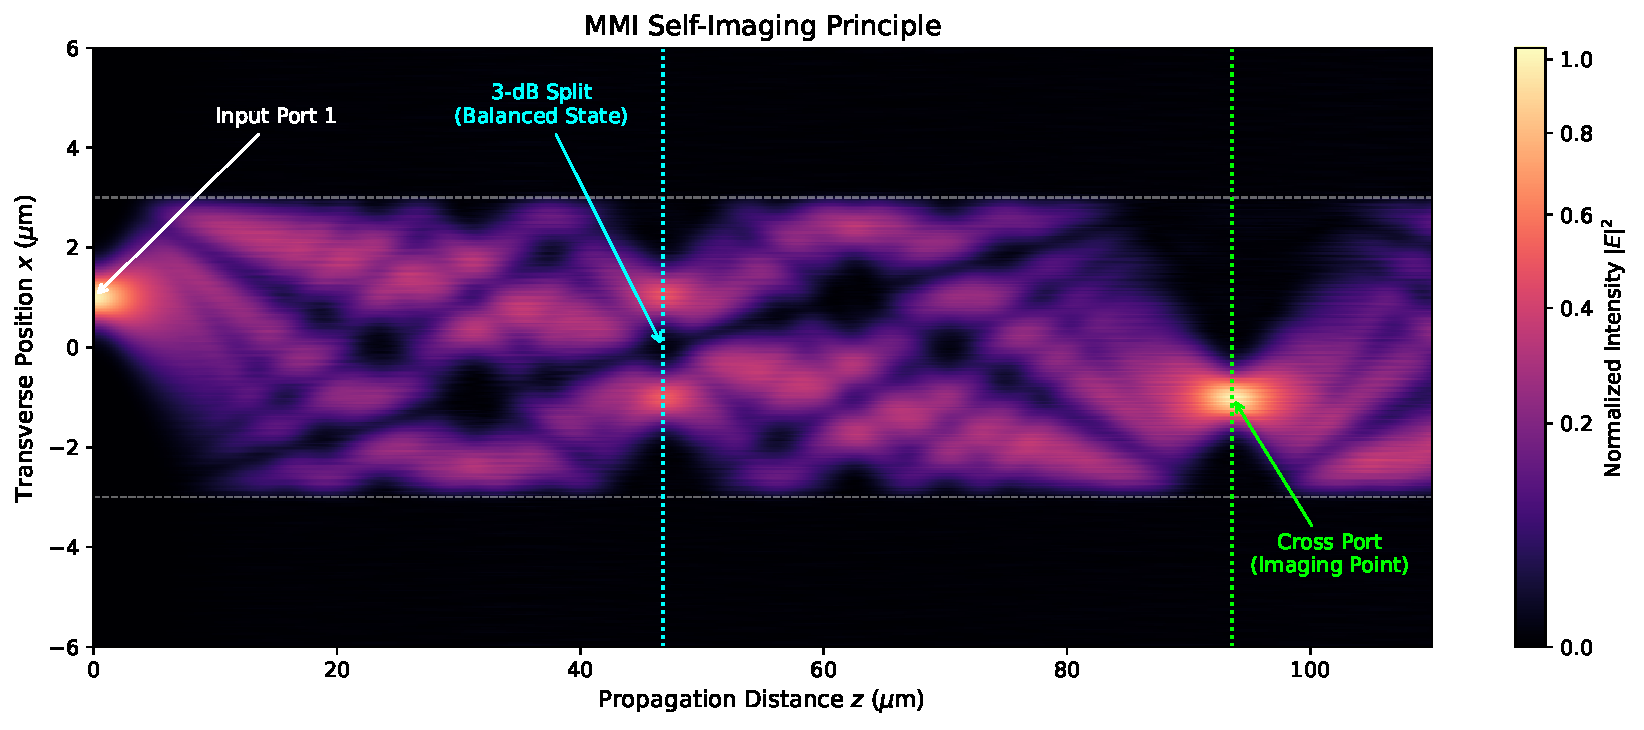
\includegraphics[width=\textwidth]{figures/ch2-mmi_2x2_self_imagin.pdf}
    \caption{BPM simulation of a $2\times2$ MMI. Vertical markers indicate the numerically 
    calibrated 3-dB splitting ($L_{\pi}/2$) and cross-over ($L_{\pi}$) imaging planes.}
    \label{fig:ch2-mmi_2x2_self_imagin}
\end{figure}

In the context of large-scale integration, MMIs offer a significant advantage in terms of 
\textit{fault tolerance} compared to directional couplers. Their performance is primarily 
determined by the width of the multimode interference region; since $W_e$ is typically several 
micrometers wide, nanometric lithographic variations represent a much smaller relative error than 
in the narrow gaps of directional couplers. Consequently, MMIs exhibit superior robustness against 
fabrication tolerances and wavelength fluctuations, ensuring a more stable power splitting ratio 
(lower imbalance) across the chip \cite{soldanoOpticalMultimodeInterference1995}. While they 
require a larger footprint and may introduce slightly higher insertion losses due to mode mismatch 
at the junctions, their reliability makes them the preferred choice for the static backbone of 
programmable photonic meshes.

\FloatBarrier

% \subsubsection*{Waveguide Crossings}

% Waveguide crossings enable optical routing in two-dimensional layouts, allowing waveguides to 
% intersect without requiring additional layers. They are particularly important in programmable 
% meshes, where dense interconnections are necessary.

% A simple orthogonal crossing introduces scattering losses and crosstalk due to modal mismatch and 
% radiation at the intersection region. Advanced crossing designs incorporate tapering, optimized 
% geometry, or multi-mode interference regions to reduce insertion loss and minimize inter-channel 
% coupling.

% In large-scale programmable circuits, even small crossing losses accumulate over multiple stages, 
% directly impacting scalability. Therefore, low-loss and low-crosstalk crossings are essential for 
% maintaining signal fidelity in deep interferometric networks.

\subsubsection*{Waveguide Crossings}

Waveguide crossings are essential for enabling complex optical routing in two-dimensional layouts, 
allowing waveguides to intersect without the need for additional lithographic layers. In 
large-scale programmable meshes, where dense interconnections and mesh-like topologies are 
required, the performance of these crossings becomes a critical factor for scalability.

A simple orthogonal intersection of two single-mode waveguides introduces significant scattering 
losses and crosstalk (typically ranging from $-20$ to $-30$ dB) due to the modal mismatch and 
radiation at the intersection region. To mitigate these effects, advanced crossing designs—such as 
those based on parabolic tapers, Bloch-mode engineering, or Multi-Mode Interference (MMI) 
regions—are employed to expand the mode and minimize field intensity at the waveguide boundaries 
during the transition.

The impact of a crossing can be modeled by its transfer matrix $\mathbf{M}_{\text{cross}}$, 
relating the throughput and the leaked (crosstalk) signals:
\begin{equation}
\begin{pmatrix} E_{out,1} \\ E_{out,2} \end{pmatrix} = \mathbf{M}_{\text{cross}} \begin{pmatrix} 
    E_{in,1} \\ E_{in,2} \end{pmatrix} = \begin{pmatrix} \tau & j\sqrt{\chi} \\ j\sqrt{\chi} & \tau 
    \end{pmatrix} \begin{pmatrix} E_{in,1} \\ E_{in,2} \end{pmatrix},
\label{eq:matrix_crossing}
\end{equation}
where $\tau$ is the complex transmission coefficient (representing insertion loss) and $\chi$ is 
the power crosstalk coefficient. 

In the context of large-scale programmable circuits, even small crossing losses ($<0.1$ dB) 
accumulate over multiple stages, directly impacting the total power budget. Furthermore, the 
coherent accumulation of crosstalk from hundreds of crossings acts as a noise floor that 
interferes with the intended signal, limiting the extinction ratio and the precision of the 
synthesized optical transformations \cite{maUltralowLossSingle2013}. Therefore, ultra-low-loss 
and low-crosstalk crossings are paramount for maintaining signal fidelity in deep interferometric 
networks.

% \textbf{Suggested figure:} Comparison between a simple crossing and an optimized crossing geometry 
% with indicated crosstalk paths.

To address the scalability limits imposed by conventional intersections, advanced designs such as 
the one proposed by Ding et al. \cite{maUltralowLossSingle2013} are employed. As illustrated in Figure 
\ref{fig:ch2-crossing_Ding_adapted}, this geometry utilizes optimized spline-based tapers to adiabatically 
expand the guided mode before the intersection. By increasing the mode field diameter, the optical 
intensity at the waveguide corners is significantly reduced, which suppresses scattering and 
minimizes crosstalk to levels below $-37$ dB with insertion losses as low as $0.028$ dB. Such 
high-performance characteristics are fundamental for the fault-tolerant operation of large-scale 
meshes, ensuring that the cumulative noise floor remains below critical thresholds for optical 
signal processing.

\begin{figure}[htbp]
    \centering
    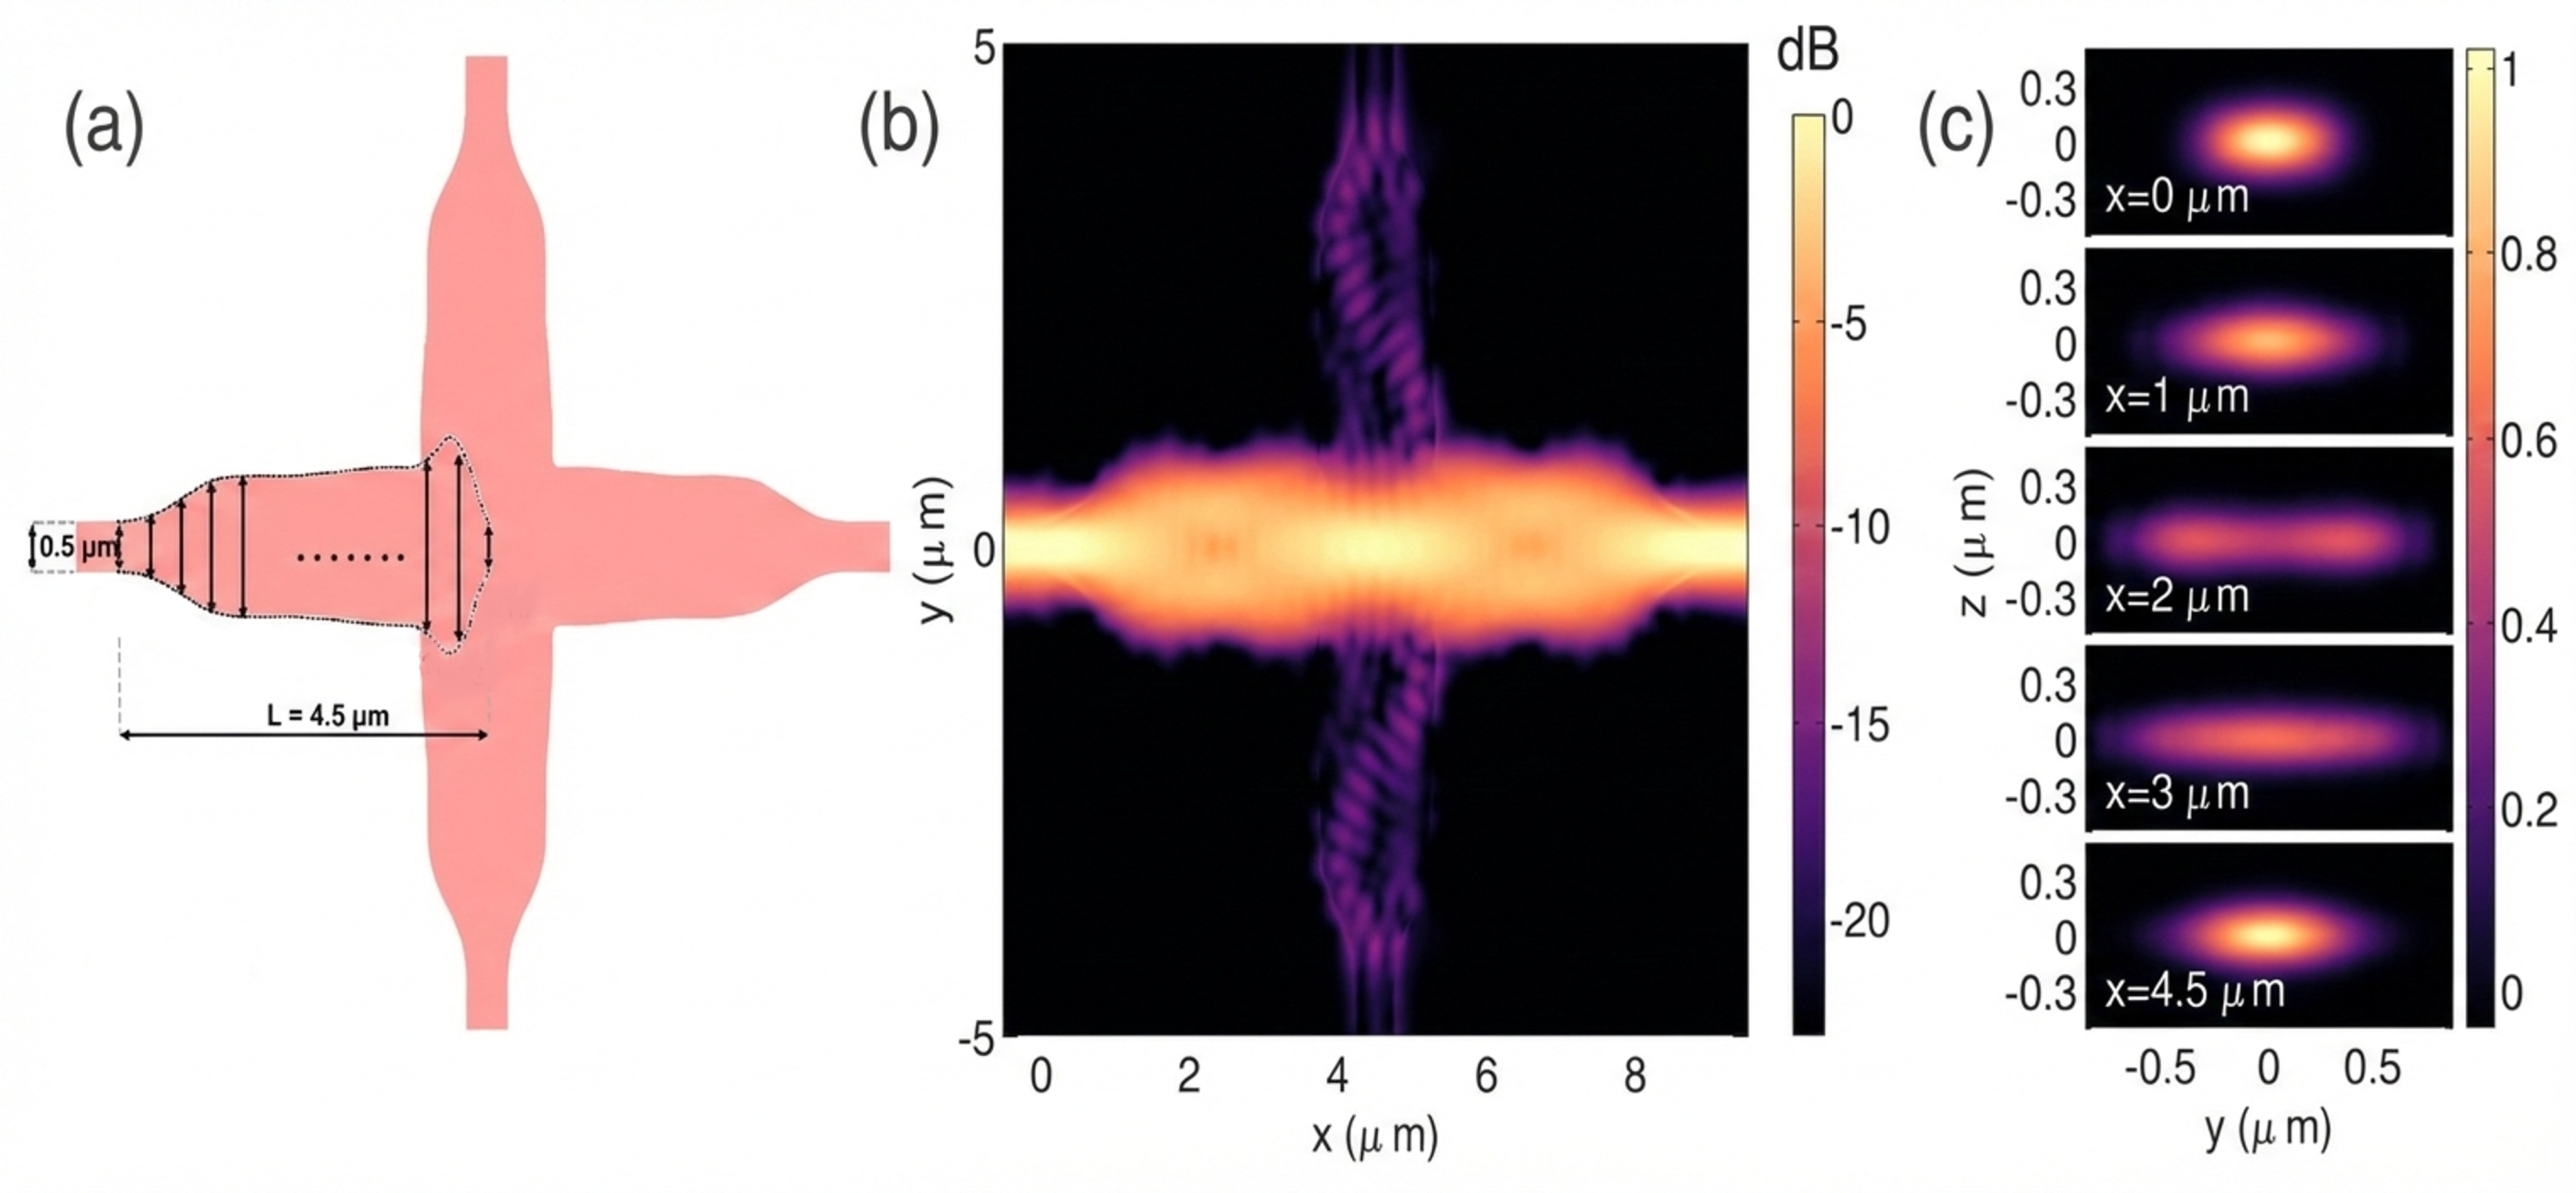
\includegraphics[width=\textwidth]{figures/ch2-crossing_Ding_adapted} 
    \caption{Optimized silicon waveguide crossing design. 
    (a) Layout geometry using spline-based tapers, 
    (b) electric field intensity simulation, and 
    (c) transverse mode profiles at different stages of the crossing. 
    Adapted from Ding et al. \cite{maUltralowLossSingle2013}.}
    \label{fig:ch2-crossing_Ding_adapted}
\end{figure}

\subsubsection*{Grating Couplers}

Grating couplers provide vertical coupling between optical fibers and planar waveguides. They 
operate based on diffraction from a periodic perturbation in the waveguide, enabling phase matching 
between the guided mode and an externally incident fiber mode.

The grating period $\Lambda$ must satisfy the phase-matching condition

\begin{equation}
\Lambda = \frac{\lambda}{n_{\text{eff}} - n_{\text{clad}}\sin\theta},
\end{equation}

where $\lambda$ is the operating wavelength, $n_{\text{eff}}$ is the effective index of the guided 
mode, $n_{\text{clad}}$ is the refractive index of the cladding, and $\theta$ is the fiber tilt 
angle.

Grating couplers enable wafer-scale testing and simplify packaging, although they typically 
introduce higher insertion loss compared to edge coupling techniques. Their bandwidth and 
efficiency depend strongly on etch depth, duty cycle, and apodization profile.

\textbf{Suggested figure:} Surface grating with tilted fiber positioned above the chip, indicating diffraction angle.

\subsubsection*{Edge Couplers}

Edge couplers provide lateral coupling between optical fibers and on-chip waveguides. They 
typically rely on adiabatic tapers that gradually expand the mode size of the silicon waveguide 
to better match the mode field diameter of the fiber.

By slowly varying the waveguide width over a sufficiently long taper length, scattering losses 
are minimized and high coupling efficiencies can be achieved. Unlike grating couplers, edge 
couplers offer lower insertion loss and broader bandwidth, but require polished chip facets and 
more complex packaging.

In programmable photonic processors intended for high-performance applications, edge coupling is 
often preferred when minimizing total insertion loss is critical.

\textbf{Suggested figure:} Long adiabatic taper expanding toward the chip facet and aligned optical 
fiber.


The passive building blocks described above define the structural and interferometric framework of 
programmable photonic circuits. While they do not provide tunability, they establish the coupling 
and interference pathways necessary for implementing linear optical transformations.

When combined with active phase tuning elements, these passive structures form reconfigurable 
interferometric units capable of realizing arbitrary 2x2 transformations. The integration of 
passive and active elements culminates in the definition of the Programmable Unit Cell, which 
will be introduced after discussing the mechanisms enabling dynamic phase control.




\subsection{Active Tuning Mechanisms}

Active tuning mechanisms provide the dynamic control required for programmable photonic operation. While passive structures define fixed coupling and interference pathways, active elements enable external electrical control over the effective refractive index or absorption of guided modes. By inducing controlled phase shifts within interferometric structures, they allow the realization of arbitrary linear optical transformations.

In silicon photonics, tunability is primarily achieved by exploiting physical mechanisms that modify the refractive index of silicon. The most relevant approaches are based on the thermo-optic effect and the plasma dispersion effect. Alternative electro-optic mechanisms may also be employed in hybrid or heterogeneous platforms.


\subsubsection*{Thermo-Optic Phase Shifters}

The thermo-optic effect constitutes the most widely used tuning mechanism in silicon photonics. Silicon exhibits a relatively large thermo-optic coefficient,

\begin{equation}
\frac{dn}{dT} \approx 1.86 \times 10^{-4} \ \text{K}^{-1},
\end{equation}

which enables efficient phase modulation through local heating.

When a resistive heater placed above the waveguide increases the local temperature by $\Delta T$, the induced phase shift over a length $L$ is given by

\begin{equation}
\Delta \phi = \frac{2\pi}{\lambda} \frac{dn}{dT} \Delta T L,
\end{equation}

where $\lambda$ is the operating wavelength. The phase shift is therefore proportional to temperature change and interaction length.

Thermo-optic phase shifters offer several advantages:
\begin{itemize}
\item Large tuning range (multiple $2\pi$ phase shifts),
\item Simple fabrication,
\item Compatibility with standard CMOS processes.
\end{itemize}

However, they also present important limitations:
\begin{itemize}
\item Relatively high power consumption (typically mW per $\pi$ shift),
\item Limited modulation speed (kHz–MHz range),
\item Thermal crosstalk between adjacent elements.
\end{itemize}

In large programmable meshes containing hundreds or thousands of phase shifters, thermal management and power scalability become critical constraints.

\textbf{Suggested figure:} Cross-sectional view of a silicon waveguide with metallic heater above oxide cladding, indicating heat diffusion profile.


\subsubsection*{Carrier-Based Phase Shifters}

An alternative approach relies on the plasma dispersion effect, where variations in free carrier concentration modify both the refractive index and absorption coefficient of silicon. This mechanism enables significantly faster modulation compared to thermal tuning.

The refractive index variation induced by changes in electron ($\Delta N_e$) and hole ($\Delta N_h$) concentrations can be approximated by empirical relations of the form

\begin{equation}
\Delta n = - (8.8 \times 10^{-22}) \Delta N_e 
           - (8.5 \times 10^{-18}) (\Delta N_h)^{0.8},
\end{equation}

with carrier concentrations expressed in cm$^{-3}$. The negative sign indicates that increasing carrier density reduces the refractive index.

Carrier-based phase shifters are typically implemented using PN or PIN junctions embedded in the waveguide. Two primary operation modes are employed:

\begin{itemize}
\item \textbf{Carrier injection}, where forward bias increases carrier density, enabling large phase shifts but introducing additional absorption losses.
\item \textbf{Carrier depletion}, where reverse bias modifies the depletion region width, enabling faster modulation with reduced optical loss.
\end{itemize}

Compared to thermo-optic tuning, plasma dispersion phase shifters offer:
\begin{itemize}
\item Higher modulation speed (up to tens of GHz),
\item Lower static power consumption (in depletion mode),
\item Direct electrical control.
\end{itemize}

However, they introduce additional propagation loss due to free-carrier absorption and require more complex fabrication processes involving doping and electrical isolation.

\textbf{Suggested figure:} Lateral PN junction integrated within a rib waveguide, showing depletion region and applied voltage.

\subsubsection*{Electro-Optic and Hybrid Approaches}

Silicon lacks a strong linear electro-optic (Pockels) effect due to its centrosymmetric crystal structure. Consequently, pure silicon platforms cannot exploit direct electric-field-induced refractive index changes.

To overcome this limitation, hybrid or heterogeneous integration with materials exhibiting strong electro-optic coefficients, such as lithium niobate or certain polymers, has been investigated. In such configurations, phase modulation can be achieved through the Pockels effect,

\begin{equation}
\Delta n = -\frac{1}{2} n^3 r E,
\end{equation}

where $r$ is the electro-optic coefficient and $E$ is the applied electric field.

These approaches enable ultra-fast and low-loss modulation, but at the expense of increased fabrication complexity and reduced compatibility with standard silicon processes. For large-scale programmable photonic processors, thermo-optic and carrier-based mechanisms remain the most widely adopted solutions.


\subsubsection*{Performance Trade-Offs and Scalability}

The choice of tuning mechanism directly impacts the scalability of programmable photonic circuits. As the number of active elements increases, cumulative power consumption, electrical routing density, and thermal management become limiting factors.

Thermo-optic tuning scales poorly in power for very large meshes due to static power requirements, whereas carrier-based approaches introduce additional optical loss that accumulates across multiple interferometric stages. The trade-off between tuning efficiency, modulation speed, insertion loss, and fabrication complexity must therefore be carefully balanced depending on the target application.

In practical implementations, programmable photonic processors often integrate monitoring photodiodes within the circuit to enable feedback-based calibration. This closed-loop control becomes essential to compensate for thermal drift, fabrication variability, and environmental fluctuations.


When integrated within interferometric configurations, active phase shifters enable continuous control over optical interference. By combining passive coupling structures with tunable phase elements, it becomes possible to implement fully controllable 2×2 linear optical transformations.

This reconfigurable interferometric element constitutes the fundamental unit of programmability in photonic circuits and is formally defined as the Programmable Unit Cell (PUC), which will be described in the following subsection.




\section{Architectures of programmable waveguide meshes}
\subsection{Mesh topologies}
% % Comparativa de geometrías.
% % Forward-only meshes (Redes alimentadas hacia adelante): Triangular, Rectangular. Estructuras que no permiten bucles de realimentación fácilmente.
% % Recirculating meshes (Redes recirculantes): Hexagonal, Triangular. Permiten sintetizar cavidades y anillos resonadores (importante para "Large-Scale").
\subsection{Circuit synthesis and routing}
% % Cómo se "programa" un circuito lógico sobre la malla física. Concepto de enrutamiento de luz por software.

\section{Challenges in large-scale integration: sources of error}
\subsection{Fabrication tolerances and process variations}
% % Variaciones estocásticas en el ancho y altura de las guías de onda (wafer thickness variations, etching errors). Cómo esto afecta al índice efectivo 
% % y desbalancea los MZIs.

\subsection{Component non-idealities}

\subsection{Yield vs. Scale}
% % Explicación estadística: a medida que aumenta el número de componentes (N), la probabilidad de tener un circuito 100% funcional decae 
% % exponencialmente sin tolerancia a fallos.


\section{State of the Art: Calibration and fault tolerance techniques}

\subsection{Automated calibration strategies}
% % Métodos actuales para caracterizar cada MZI individualmente (algoritmos de optimización, monitores de potencia integrados).

\subsection{Redundancy and reconfiguration}
% % Uso de caminos alternativos en la malla para esquivar componentes rotos (re-routing).

\subsection{Hardware-level fault tolerance}
% % Diseños de acopladores robustos o componentes de banda ancha que son menos sensibles a errores de fabricación (Aquí es donde probablemente 
% % encajará tu contribución en capítulos posteriores).








% \chapter{Fundamentals and State of the Art of Programmable Integrated Photonics} \label{chap:fundamentals}

% \section{Fundamentals of Integrated Photonics}
% Integrated photonics aims to generate, guide, manipulate, and detect optical signals within a compact
% and scalable platform by integrating multiple photonic components on a single substrate. By leveraging 
% waveguiding structures with high refractive index contrast, integrated photonic circuits enable strong 
% optical confinement and precise control of light propagation over centimeter-scale distances within 
% chip-scale footprints. This approach provides a robust and reproducible alternative to bulk and 
% fiber-based optical systems, while benefiting from wafer-scale fabrication and compatibility with 
% semiconductor manufacturing processes\cite{sorefPresentFutureSilicon2006,thomsonRoadmapSiliconPhotonics2016}.

% The fundamental building block of integrated photonics is the optical waveguide, which confines light 
% through total internal reflection or effective index guiding mechanisms. In most integrated platforms, 
% waveguides consist of a high-index core surrounded by lower-index cladding materials, enabling single-mode 
% or multi-mode propagation depending on geometry and wavelength. The propagation of light along a waveguide 
% mode is commonly described in terms of its propagation constant $\beta$, which is related to the effective 
% refractive index $n_{\mathrm{eff}}$ as

% \begin{equation}
% \beta = k_0 n_{\mathrm{eff}},
% \end{equation}

% where $k_0 = 2\pi / \lambda$ is the free-space wavenumber and $\lambda$ is the optical wavelength. The 
% accumulated optical phase over a waveguide section of length $L$ is therefore given by

% \begin{equation}
% \phi = \beta L = \frac{2\pi}{\lambda} n_{\mathrm{eff}} L.
% \end{equation}

% This phase accumulation constitutes the physical basis of interferometric devices and phase-tunable 
% photonic circuits, which are central to reconfigurable and programmable photonic integrated systems.

% The fundamental building blocks of integrated photonics are summarized in 
% Fig.~\ref{fig:ch2-photonics_summary}, including waveguide confinement and guided modes,
% basic passive components, and representative interferometric and resonant structures.

% \begin{figure}[t]
%     \centering
%     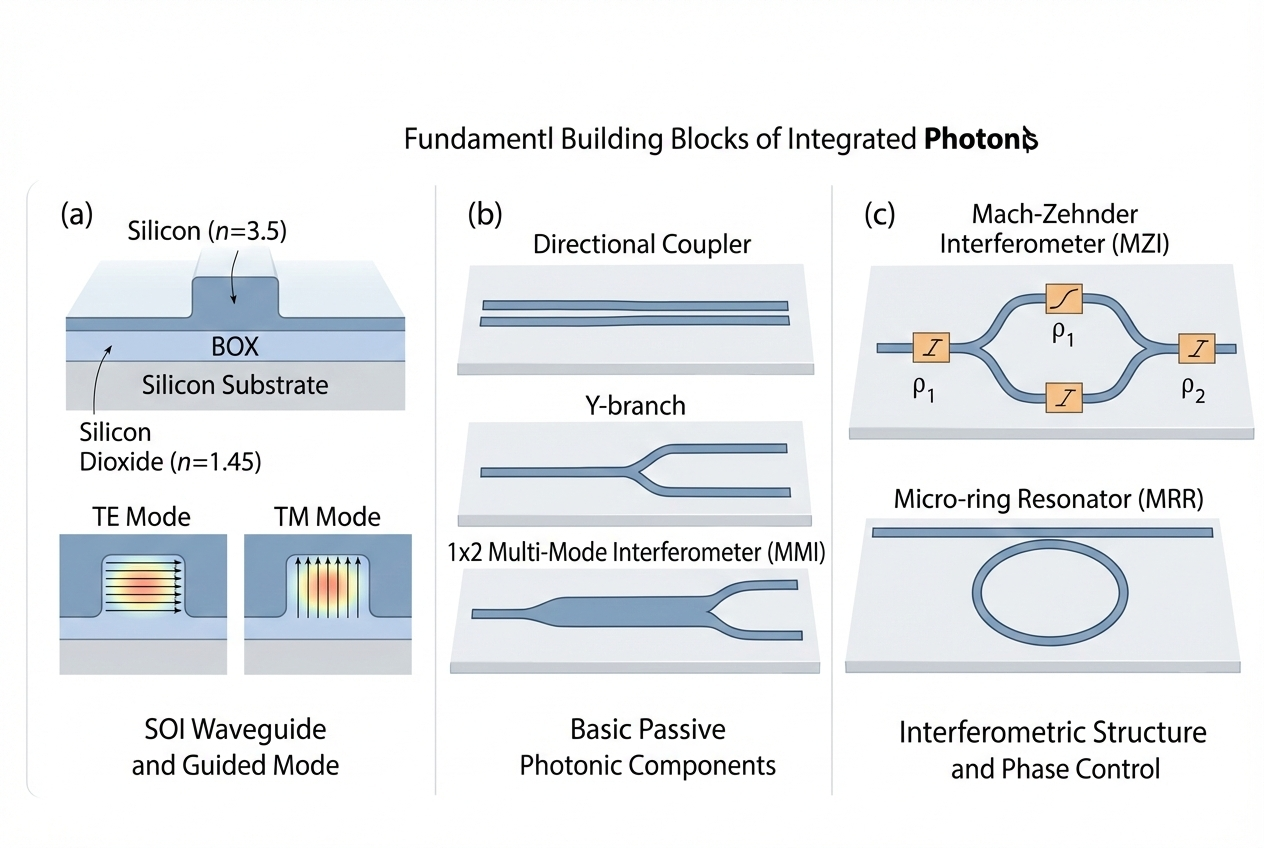
\includegraphics[width=\linewidth]{figures/ch2-photonics_summary.png}
%     \caption{Fundamental building blocks of integrated photonics. 
%     (a) Cross-section of a silicon-on-insulator (SOI) waveguide and representation 
%     of the fundamental TE and TM guided modes. 
%     (b) Basic passive photonic components including a directional coupler, 
%     a Y-branch, and a 1x2 multi-mode interferometer (MMI). 
%     (c) Mach-Zehnder interferometer (MZI) and a micro-ring resonator (MRR), 
%     which enable phase control and spectral filtering.}
%     \label{fig:ch2-photonics_summary}
% \end{figure}





% Among the various material platforms developed for integrated photonics, silicon-on-insulator (SOI) 
% technology has emerged as the most widely adopted, largely due to its high refractive index contrast, 
% mature fabrication ecosystem, and compatibility with complementary metal-oxide-semiconductor (CMOS) 
% processes\cite{sorefPresentFutureSilicon2006}. Silicon photonics enables dense integration of passive 
% components such as waveguides, bends, 
% splitters, and interferometers, as well as active devices including modulators and photodetectors. 
% Alternative platforms, such as silicon nitride and III-V semiconductors, are also widely used, offering 
% advantages in terms of lower propagation loss, broader transparency windows, or native light emission, 
% and are often combined with silicon through heterogeneous or hybrid integration approaches.

% Passive photonic components form the backbone of integrated photonic circuits and include waveguides, 
% directional couplers, multi-mode interferometers (MMIs), filters, and resonant structures. These elements 
% define the static optical paths and spectral responses of a circuit. Their performance is largely determined 
% by geometry and material properties, making them highly sensitive to fabrication variations, particularly 
% in high-index-contrast platforms. As circuit complexity increases, small deviations in waveguide dimensions 
% or coupling gaps can accumulate and significantly impact overall system performance.

% Active photonic components enable dynamic control of optical signals and are essential for reconfigurable 
% and, at a higher level, programmable photonic systems. Phase shifters and modulators exploit mechanisms 
% such as the thermo-optic 
% effect, free-carrier dispersion, or electro-optic effects to induce controlled changes in the effective 
% refractive index. Photodetectors provide electrical readout of optical signals and are critical for 
% monitoring, feedback, and control in complex circuits. The integration of active components introduces 
% additional constraints related to power consumption, speed, thermal management, and electrical interfacing, 
% which become increasingly relevant as the scale of integration grows
% \cite{millerDeviceRequirementsOptical2009}.

% Loss mechanisms play a central role in determining the scalability of integrated photonic circuits. 
% Propagation losses arising from material absorption, sidewall roughness, and scattering, as well as excess 
% losses introduced by couplers, bends, and crossings, accumulate as circuit depth increases. In large-scale 
% photonic integrated circuits, loss accumulation can limit usable circuit size and directly impact 
% signal-to-noise ratio and energy efficiency. As a result, minimizing loss at both the component and 
% architectural levels is a key design consideration, particularly for programmable photonic systems that 
% rely on cascaded interferometric structures.

% Overall, the fundamentals of integrated photonics provide the technological foundation upon which reconfigurable 
% and programmable photonic integrated circuits are built. While the integration of optical components on a single 
% chip enables compactness and scalability, it also introduces challenges related to fabrication variability, 
% loss accumulation, and active control. These aspects become increasingly critical in the context of 
% large-scale programmable photonic architectures and motivate the need for careful design methodologies and 
% robust control strategies, which are discussed in the following sections.